% Final
\section{Návrh prototypu uživatelského rozhraní}

% Final
V této sekci se zaměřím na návrh \textit{high fidelity} prototypu uživatelského rozhraní\footnote{Dostupné na: \href{https://www.figma.com/design/VZFuqWojrXq8yWjrBIq4OH}{https://www.figma.com/design/VZFuqWojrXq8yWjrBIq4OH}}, tedy prototypu, který bude obsahovat detailní návrh uživatelského rozhraní včetně definovaných stylů, barev, písma, ilustrací a interakcí \cite[53-54]{NURUIDesignSteps}. Cílem je tak vytvořit návrh uživatelského rozhraní, které bude přesně specifikovat vzhled aplikace a přechody mezi jednotlivými stránkami. Prototyp následně bude sloužit jako podklad pro samotnou implementaci aplikace.

% Final
Pro tvorbu prototypu jsem zvolil nástroj Figma\footnote{Dostupné na: \href{https://www.figma.com/}{https://www.figma.com/}}, protože umožňuje rychlé iterace návrhu, práci s komponentami a také propojení obrazovek do podoby interaktivního prototypu. Při návrhu jsem vycházel ze stylů definovaných v předchozí sekci.

% Final
\subsection{Tvorba prototypu}

% Final
V rámci mé bakalářské práce jsem se mimo jiné věnoval vytvoření návrhu uživatelského rozhraní pro původní aplikaci na výuku angličtiny \cite{Jenicek2024BachelorThesis}. V průběhu let jsem ovšem zpozoroval několik nedostatků tohoto prototypu. Použitá knihovna předdefinovaných komponentů je zbytečně složitá a komplikuje vytváření a používání nových komponentů. Prototyp také nevyužívá moderní funkce programu Figma, jako například definice globálních proměnných a proměnných komponentů. S ohledem na nově definované styly, nové funkce a na nový účel aplikace jsem se tak rozhodl vytvořit celý návrh uživatelského rozhraní od začátku a bez návaznosti na původní prototyp.

% Final
Při tvorbě prototypu jsem postupoval následovně. Nejprve jsem pomocí proměnných zadefinoval jednotlivé styly aplikace dle návrhu popsaného v předchozí sekci. Následně jsem provedl hrubý návrh základních komponent a stránek aplikace. Poté jsem se v rámci agilního procesu vývoje vždy zaměřil na jednu funkci, kterou jsem navrhl podrobněji a zprovoznil její interakce v prototypu. Po dokončení návrhu dané funkce jsem provedl její implementaci a testování, které jsou popsané v následujících kapitolách. Po dokončení dané funkce jsem se přesunul na následující funkci, dle její priority. Po dokončení návrhu všech funkcí jsem provedl závěrečné úpravy návrhu a organizaci jednotlivých stránek a komponentů.

% Final
Při návrhu jsem kladl důraz na znovupoužitelnost komponentů a na využití pokročilejších možností programu Figma, díky kterým bude možné prototyp v budoucnu jednodušeji rozšiřovat a upravovat. Konkrétně jsem široce využíval komponenty a jejich varianty, díky kterým je zajištěna vyšší konzistence samotného návrhu. Dále jsem využíval lokální proměnné komponentů a globální kolekce proměnných, díky kterým je možné kdykoliv měnit styly v celém návrhu, aniž by bylo nutné modifikovat samotné stránky a komponenty \cite{FigmaVariablesGuide}. 

% Final
Jednotlivé komponenty jsem dále strukturoval tak, aby bylo možné je přímo implementovat s využitím jejich zadefinovaných parametrů v prototypu. Při návrhu jsem také často využíval funkci \textit{auto layout}, díky které je možné přesně specifikovat rozložení komponentů tak, aby byly responzivní a použitelné v různých částech UI \cite{FigmaAutolayoutGuide}.

% Final
Jako součást návrhu jsem také vytvořil dva režimy rozhraní aplikace, světlý a tmavý. Oba režimy sdílí stejné rozvržení stránek a komponentů a liší se pouze aplikovanými styly, zejména barvami pozadí, textu a stavů. Pro definici světlého a tmavého režimu jsem využil funkci módů proměnných \cite{FigmaModesForVariables}, díky které je možné pro každý režim definovat jiné hodnoty proměnných a následně snadno mezi jednotlivými režimy přepínat. Díky tomu byla opět zajištěna vyšší konzistence návrhu, jelikož není třeba pro světlý a tmavý režim navrhovat samostatné stránky, ale je možné pouze přepínat mezi aplikovanými styly.

% Final
Vytvořený návrh vzhledu jsem také doplnil o interakce odpovídající reálnému používání aplikace. Zaměřil jsem se zejména na navigaci mezi obrazovkami tak, aby bylo možné procházet základní scénáře používání aplikace. Díky tomu bylo možné prototyp interaktivně procházet, což mi umožnilo odhalit různé nedostatky v návrhu ještě před zahájením implementace.

% Final
Pro ukázku návrhu jsem vybral několik stránek z prototypu. Tyto stránky lze nalézt na obrázcích \ref{fig:navrh-1}, \ref{fig:navrh-2}, \ref{fig:navrh-3} a \ref{fig:navrh-4}.

% Review
\begin{figure}[!ht]
    \centering
    \begin{minipage}{0.45\textwidth}
        \centering
        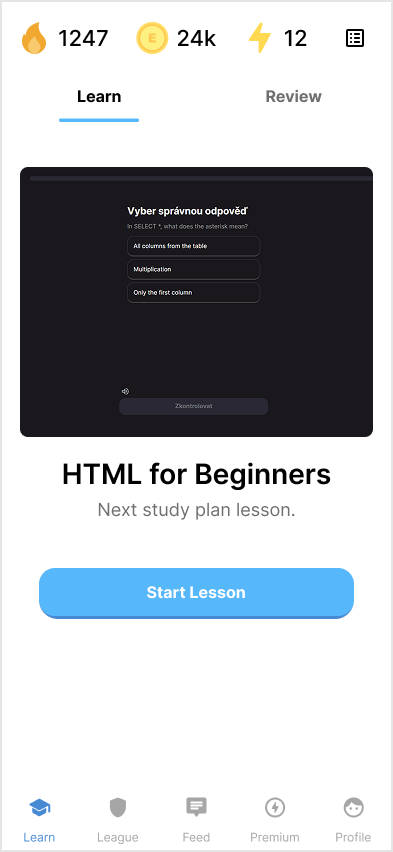
\includegraphics[width=\textwidth]{./images/home [learn-section].png}
        \caption{Ukázka návrhu hlavní stránky aplikace}
        \label{fig:navrh-1}
    \end{minipage}
    \hfill
    \begin{minipage}{0.45\textwidth}
        \centering
        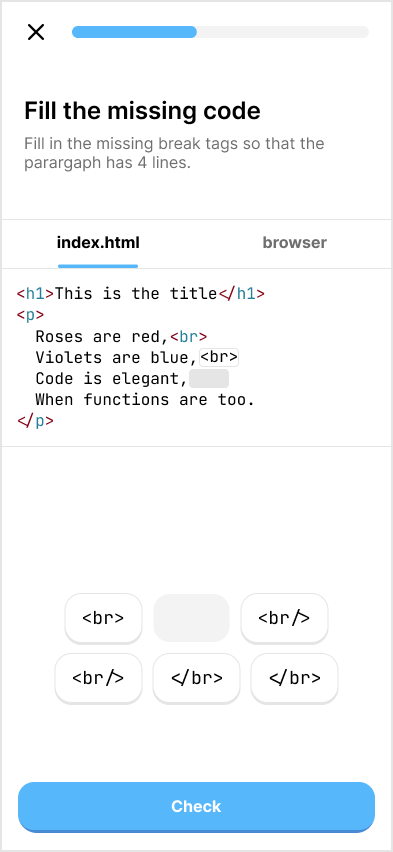
\includegraphics[width=\textwidth]{./images/study-session [fill in code].png}
        \caption{Ukázka návrhu cvičení programování}
        \label{fig:navrh-2}
    \end{minipage}
\end{figure}

% Review
\begin{figure}[!ht]
    \centering
    \begin{minipage}{0.45\textwidth}
        \centering
        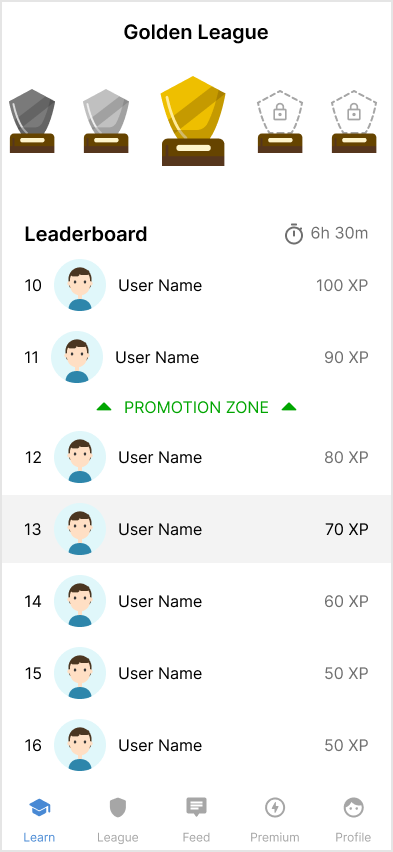
\includegraphics[width=\textwidth]{./images/leaderboard.png}
        \caption{Ukázka návrhu žebříčku uživatelů}
        \label{fig:navrh-3}
    \end{minipage}
    \hfill
    \begin{minipage}{0.45\textwidth}
        \centering
        
\includegraphics[width=\textwidth]{./images/user.png}
        \caption{Ukázka návrhu uživatelského profilu}
        \label{fig:navrh-4}
    \end{minipage}
\end{figure}

% Final
\subsection{Responzivita}

% Final
Návrh prototypu jsem realizoval přístupem \textit{mobile-first} \cite{MobileFirst}. Primární cílovou platformou této aplikace jsou mobilní zařízení, proto jsem nejprve navrhl vzhled stránek pro menší rozlišení a teprve následně jsem řešil úpravy pro větší displeje. Tento postup mi umožnil soustředit se na efektivní využití prostoru a na jednoduché rozvržení stránek, které je na malých obrazovkách klíčové.

% Final
Při návrhu prototypu bylo třeba rozhodnout, jakým způsobem bude rozhraní responzivní, tedy jak se bude rozložení stránek přizpůsobovat různým velikostem displeje. Při návrhu responzivity je možné využít několik standardních rozložení stránek. 

% Final
Rozložení \textit{mostly fluid} například typicky pracuje s bloky obsahu, které se přesouvají pod sebe se zmenšující se velikostí obrazovky \cite[7]{NURResponsiveDesign}. Dále je možné využít rozložení \textit{column drop}, které využívá několik sloupců s obsahem a se zmenšující se obrazovkou se sloupce opět přesouvají pod sebe \cite[8]{NURResponsiveDesign}. Také je možné využít rozložení \textit{layout shifter}, které představuje nejkomplexnější ze zmíněných přístupů a spočívá v navržení různé struktury stránek pro každou velikost displeje \cite[9]{NURResponsiveDesign}. 

% Final
V tomto projektu jsem se rozhodl využít přístup \textit{tiny tweaks}, který spočívá v uspořádání veškerého obsahu stránky do jediného sloupce a zachování tohoto rozložení stránky napříč všemi zařízeními \cite[10]{NURResponsiveDesign}. Na stránkách jsou tak při změně velikosti displeje provedeny pouze drobné úpravy ve velikostech jednotlivých komponentů. Implementace se tak bude řídit primárně návrhem pro mobilní zařízení a na větších displejích se budou měnit především maximální šířka obsahu, odsazení a práce s volným prostorem. Kromě toho bude struktura stránek zachována a bude napříč zařízeními stejná.

% Final
Jako důsledek zvolení tohoto přístupu je tak možné udržet návrh jednoduchý a konzistentní. Zároveň díky totožnému rozložení stránek je snížené riziko rozdílného chování napříč různými velikostmi displejů. Aplikaci by tak mělo být snazší rozšiřovat, udržovat a testovat.

% Final
\subsection{Testování a upravování prototypu}

% Final
Prototyp jsem průběžně manuálně testoval, upravoval a zdokonaloval. Při testování a procházení prototypu jsem se snažil zachytit základní problémy v použitelnosti a nekonzistenci návrhu a identifikovat tak nedostatky návrhu ještě před samotnou implementací.

% Final
Návrh jsem se pak snažil průběžně upravovat tak, aby lépe odpovídal očekávaným potřebám uživatelů a aby byl v souladu se zavedenými zásadami designu. Při upravování návrhu jsem se zaměřoval zejména na to, aby návrh splňoval 10 základních heuristik použitelnosti UI definovaných Jakobem Nielsenem \cite{Nielsen10Heuristics}. Výsledná aplikace by tak měla být pro uživatele lépe použitelná.
